
\textbf{Ejemplo 1}\\
Supongamos que para realizar un proyecto se necesita realizar una inversión inicial de 80.000 COP y otra inversión de 45.000 COP al final del primer mes, en los meses 2 y 3 los ingresos son equivalentes a los egresos pero a partir del mes 4 se producen ingresos así: mes 4 30.000 COP, mes 5 50.000 COP, mes 6 60.000 COP. Determinar si el proyecto lo pueden realizar los inversionistas A o B mencionados anteriormente. Suponga una TIO para el inversionista A del 3\% período mes vencido y para el inversionista B del 2\% período mes vencido.\\



%%%%%%%%%%%%%%%%%%% EJERCICIO 1 %%%%%%

%\newpage %USAR SOLO SI EL SOLUCION QUEDA SOLO Y ES NECESARIO BAJARLO A LA SIGUIENTE PAGINA
\textbf{Solución.}\\
%La tabla ira centrada
\begin{center}
	\renewcommand{\arraystretch}{1.5}% Margenes de las celdas
	%Creacion de la cuadricula de 3 columnas \end{flushleft}
	\begin{longtable}[H]{|C{0.3\linewidth}|C{0.3\linewidth}|C{0.3\linewidth}|}
		%Creamos una linea horizontal
		\hline
         %%%%% INICIO FLUJO DE CAJA
		\rowcolor[HTML]{FFB183}
		\multicolumn{3}{|c|}{\cellcolor[HTML]{FFB183}\textbf{1. Asignación periodo focal}}   \\ \hline
		\multicolumn{3}{|c|} {$pf: 0 pv$} \\ \hline
		%%%%%%%%%% FIN TITULO
		%%%%%%%%%% INICIO TITULO
		%Lo que se hace aqui es mezclar las 3 columnas en una sola
		\multicolumn{3}{|c|}{\cellcolor[HTML]{FFB183}\textbf{2. Declaración de variables}}   \\ \hline
		\multicolumn{1}{|c|}{\cellcolor[HTML]{FFB183}\textbf{Variables monetarias}}                   & \multicolumn{1}{|c|}{\cellcolor[HTML]{FFB183}\textbf{Variables Conceptuales}}                   & \multicolumn{1}{|c|}{\cellcolor[HTML]{FFB183}\textbf{Variables incógnitas}}                                                                         \\ \hline

		%%%%%%%%%% FIN TITULO
		%%%%%%%%%% INICIO DE MATEMATICAS
		%Cada & hace referencia al paso de la siguiente columna

		$P_{0} = -80{.}000COP(P=Egresos)$ & $i_{a} = TIO_{a} = 3\%pmv \equiv 0,03 pmv$ & $VPN_{A}= ? COP$ \\[1em]
		$P_{1} = -45{.}000COP$ & $i_{b} = TIO_{b} = 2\%pmv \equiv 0,02 pmv$ & $VPN_{B}= ? COP$ \\[1em]
		$F_{1} = 30{.}000COP(F=Ingresos)$ & $n_{a} = n_{b} = 6 pmv$ & \\[1em]
		$F_{2} = 50{.}000COP$ & $n_{1} = 1 pmv$ & \\[1em]
		$F_{3} = 60{.}000COP$ & $n_{2} =  4 pmv$ & \\[1em]
		 & $n_{3} = 5 pmv$ & \\[1em]
		 & $n_{4} = 6 pmv$ &
        
        \\\hline

		%%%%%%%%%% FIN DE MATEMATICAS
		%%%%% FIN DECLARACION DE VARIABLES


		%%%%% INICIO FLUJO DE CAJA
		\rowcolor[HTML]{FFB183}
		\multicolumn{3}{|c|}{\cellcolor[HTML]{FFB183}\textbf{3. Diagrama de flujo de caja}} \\ \hline
		%Mezclamos 3 columnas y ponermos el dibujo
		%%%%%%%%%%%%% INSERCION DE LA IMAGEN
		%Deberan descargar las imagenes respectivas del drive y pegarlas en la carpeta
		%n_capitulo/img/ejemplos/1/capitulo1ejemplo1.pdf  (el /1/ es el numero del ejemplo)
		\multicolumn{3}{|c|}{ 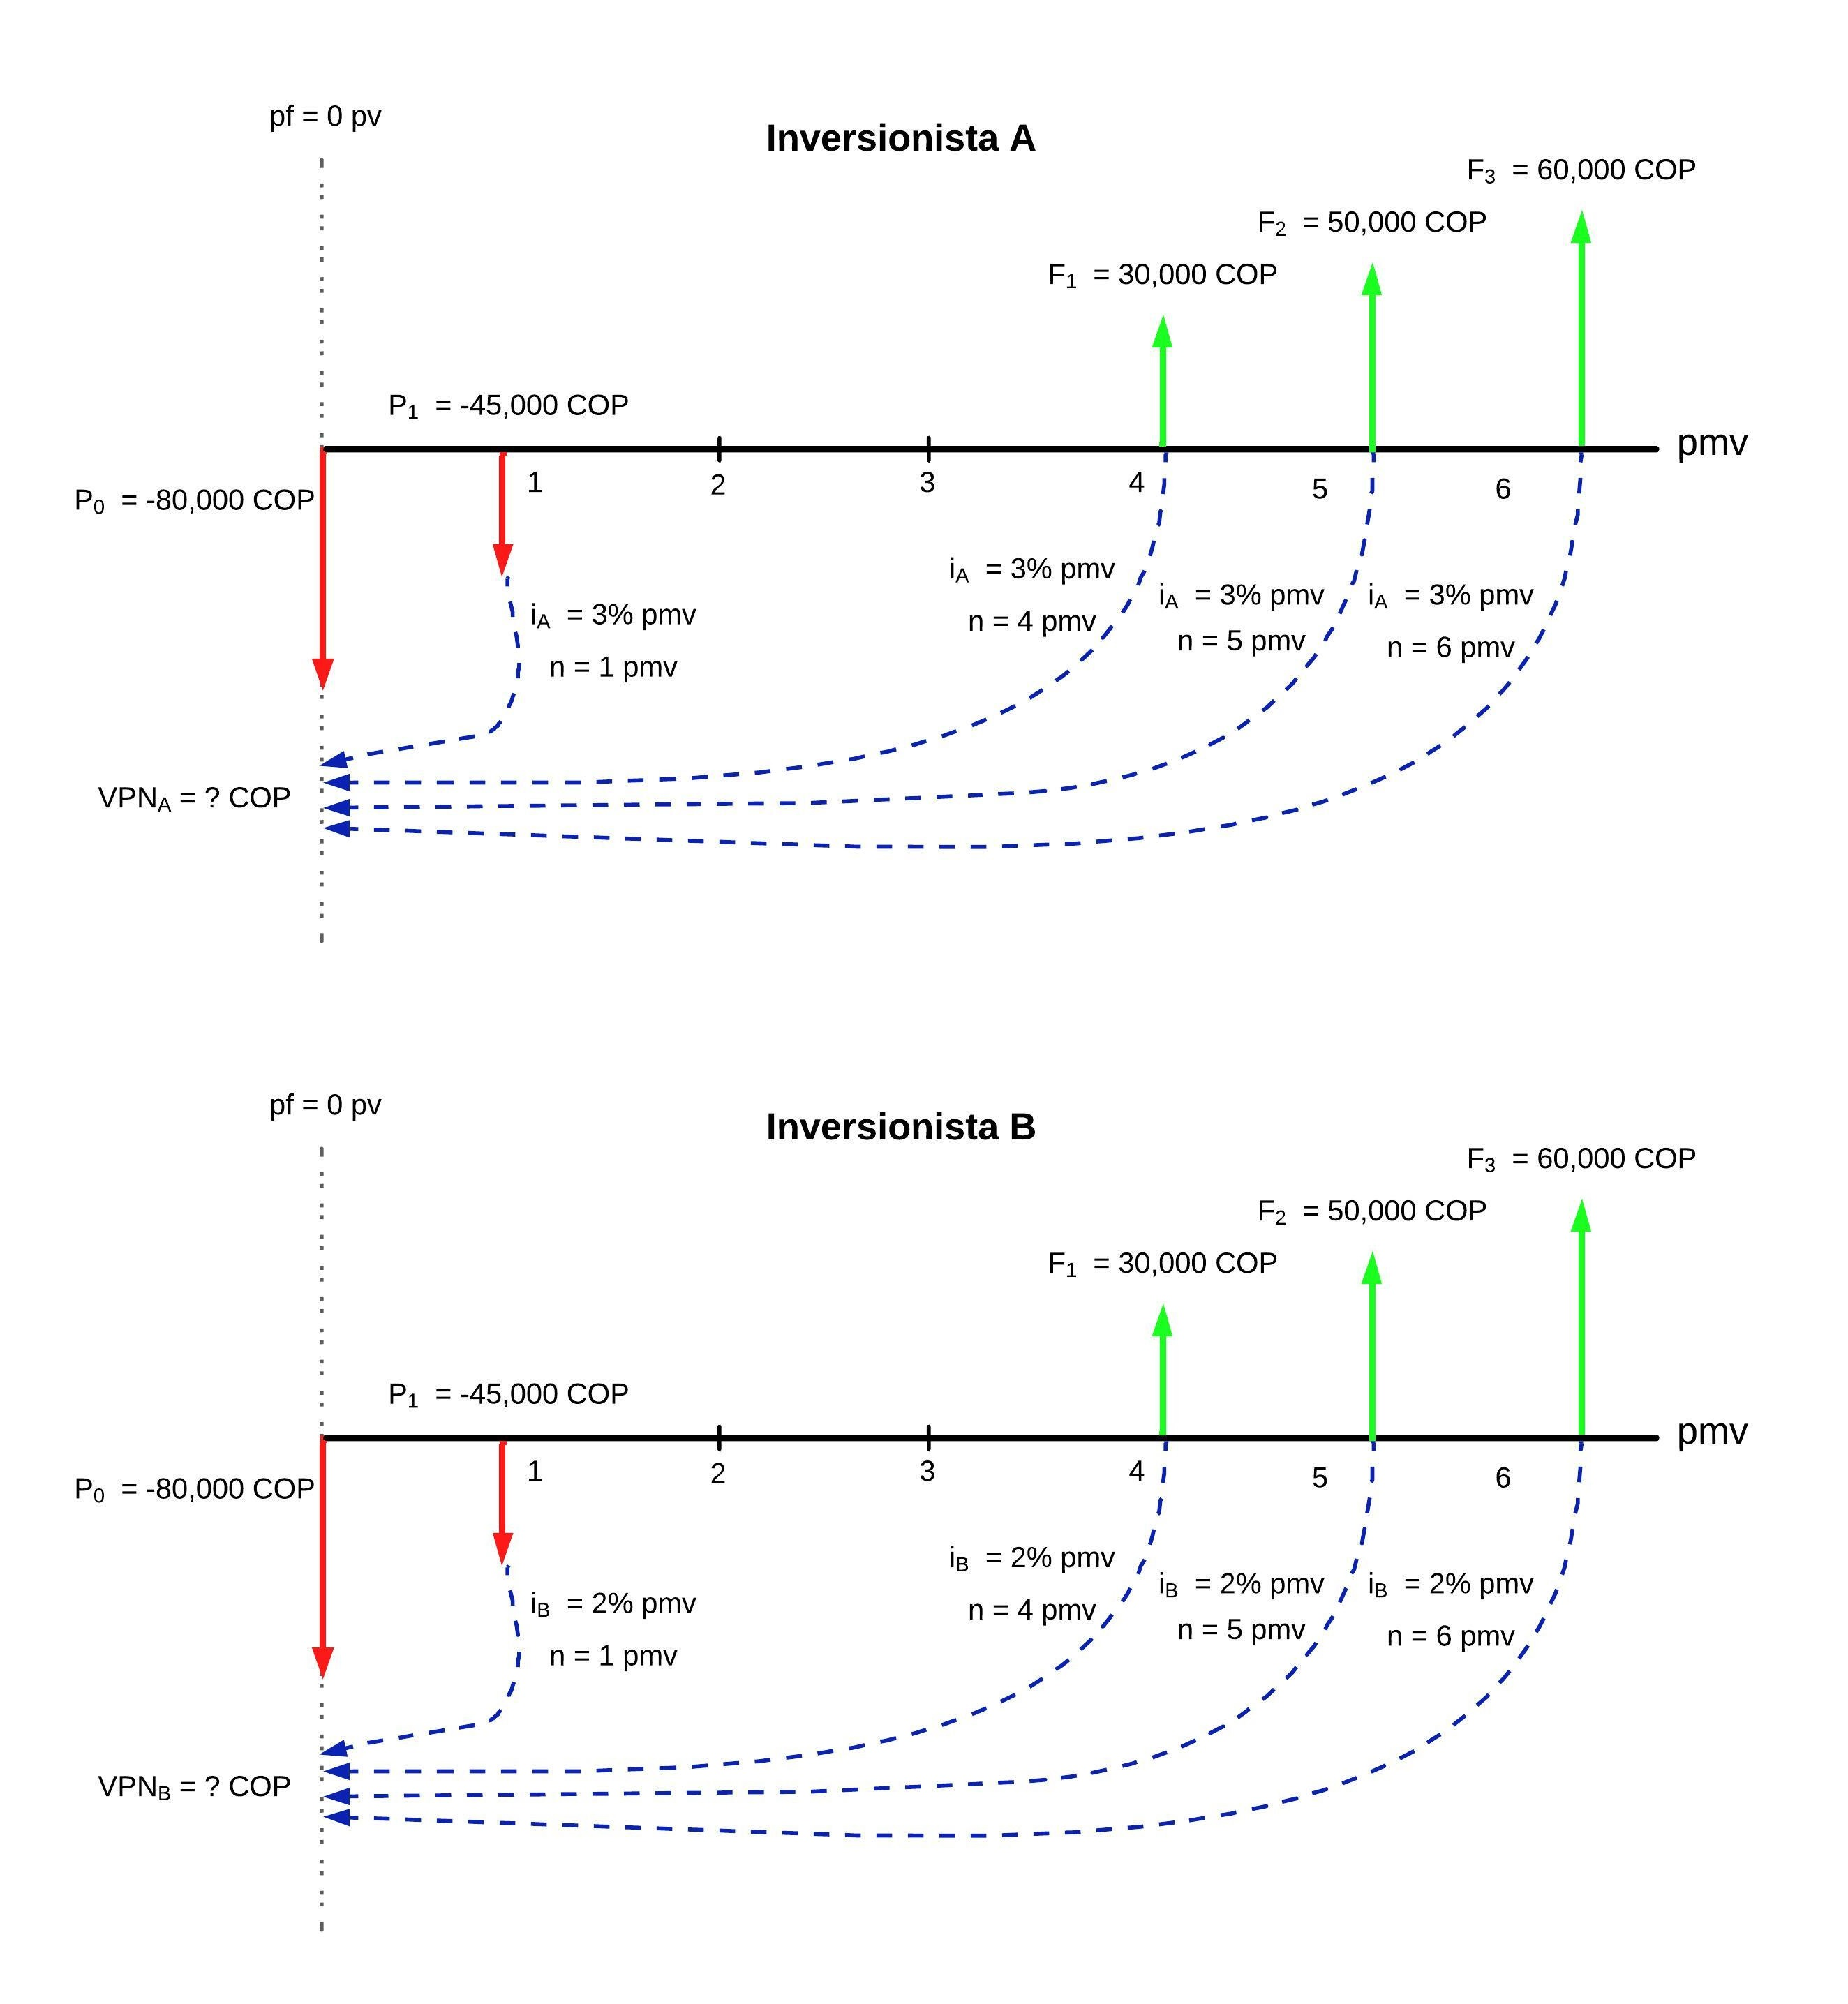
\includegraphics[trim=-5 -5 -5 -5 , scale=1,width=380px, height=450px]{9_Capitulo/ejemplos/1/exportados/DiaCEjem1Cap9(1).png} }   \\ \hline
		%%%%%%%%%%%%% FIN INSERCION DE IMAGEN
		%%%%%FIN FLUJO DE CAJA



		%%%%% INICIO DECLARACION FORMULAS
		%%%%%%%%%%% INICIO TITULO
		\rowcolor[HTML]{FFB183}
		\multicolumn{3}{|c|}{\cellcolor[HTML]{FFB183}\textbf{4. Declaración de fórmulas}}    \\ \hline
		%%%%%%%%%%% FIN TITULO
		%%%%%%%%%%% INICIO MATEMATICAS
		\multicolumn{3}{|c|}{$\sum F_{n}(1+i)^{-n} $\hspace{0.3cm} \textit{Valor presente neto}} \\ \hline
		%%%%%%%%%% FIN MATEMATICAS
		%%%%%% INICIO DESARROLLO MATEMATICO
		\rowcolor[HTML]{FFB183}
		%%%%%%%%%%INICIO TITULO
		\multicolumn{3}{|c|}{\cellcolor[HTML]{FFB183}\textbf{5. Desarrollo matemático}}       \\ \hline
		%%%%%%%%%% FIN TITULO
		%%%%%%%%%% INICIO MATEMATICAS
		\multicolumn{3}{|c|}{$VPN_{a} = -80{.}000COP(1+0pmv)^{-0pmv} - 45{.}000COP(1+0.03pmv)^{-1pmv} $} \\
        \multicolumn{3}{|l|}{$+ 30{.}000COP(1+0.03pmv)^{-4pmv} + 50{.}000COP(1+0.03pmv)^{-5pmv} + 60{.}000COP(1+0.03pmv)^{-6pmv}$}
        \\
		\multicolumn{3}{|c|}{$VPN_{a} = -3{.}655COP$} \\
		\multicolumn{3}{|c|}{$VPN_{b} = -80{.}000COP(1+0pmv)^{0pmv} - 45{.}000COP(1+0.02pmv)^{-1pmv}$} \\
        \multicolumn{3}{|l|}{$+ 30{.}000COP(1+0.02pmv)^{-4pmv} + 50{.}000COP(1+0.02pmv)^{-5pmv} + 60{.}000COP(1+0.02pmv)^{-6pmv}$} \\ \multicolumn{3}{|c|}{$VPN_{b} = 2{.}162COP$} \\ \hline

		%%%%%%%%%% FIN MATEMATICAS
		%%%%%% FIN DESARROLLO MATEMATICO
		%%%%%% INICIO RESPUESTA
		\rowcolor[HTML]{FFB183}
		%%%%%%%%%%INICIO TITULO
		\multicolumn{3}{|c|}{\cellcolor[HTML]{FFB183}\textbf{6. Respuesta}}   \\ \hline
		%%%%%%%%%% FIN TITULO
		%%%%%%%%%% INICIO RESPUESTA MATEMATICA
        \multicolumn{3}{|c|}{En un proyecto llevado a cabo por dos inversionistas A y B, se tiene:}  \\
        \multicolumn{3}{|c|}{Para el inversionista A, VPN < 0, es decir que, no se recomienda realizar el proyecto} \\
        \multicolumn{3}{|c|}{Para el inversionista B, VPN > 0, es decir que, se recomienda realizar el proyecto} \\ \hline

		%%%%%%%%%% FIN MATEMATICAS
		%%%%%% FIN RESPUESTA
	\end{longtable}
	%Se crean dos lineas en blanco para que no quede el siguiente texto tan pegado
	%\newline \newline %USARLO SI CREES QUE ES NECESARIO
\end{center}
%%%%%%%%%%%%%%%%%%%%%%%%%%FIN EJERCICIO 1 %%%%%%%%%%%%%%%%%%%%%%%%%%%
